\documentclass[a4paper,12pt]{article}
\usepackage[utf8]{inputenc}
\usepackage[T1]{fontenc}
\usepackage[british]{babel}
\usepackage{hyperref}
\usepackage{listings}
\usepackage{xspace}
\usepackage{graphicx}
\usepackage{indentfirst}

\title{Gomat specification}
\author{Gauthier Jolly \and K\'{e}vin Car\'{e}nou \and Matei Oltean}

\newcommand{\Gossiper}{\texttt{Gossiper}\xspace}
\newcommand{\Gomat}{\texttt{Gomat}\xspace}
\newcommand{\Go}{\texttt{Go}\xspace}

\begin{document}
\maketitle
\tableofcontents
\newpage
    \section{Introduction}
    \Gomat is a tool which allows users to compute complex operation on matrices on a computer network.
    \Gomat is in the same time a \texttt{Go API} and a daemon. By running the daemon, a user becomes part of a network and can use the \texttt{Go API} to execute big computations.

    \section{Goal and Functionalities}
        \subsection{Daemon}
    When a user wants to join a \Gomat network, it has to run the dedicated daemon. The daemon is the main component of the application. It splits and merges, executes computations and communicates with other peers. For this last point, it uses a \Gossiper network.

        \subsubsection{GUI}
        \begin{figure}[!ht]
            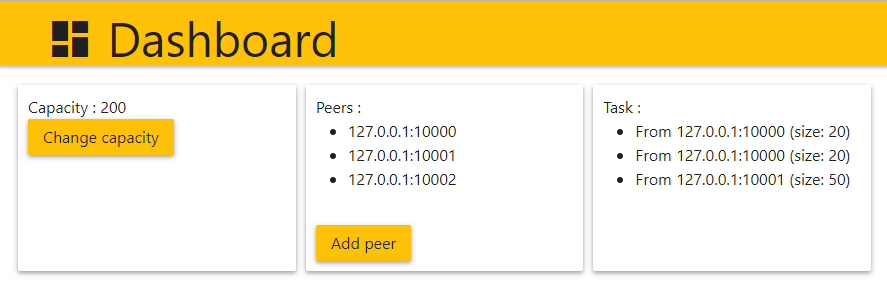
\includegraphics[width=.95\textwidth]{gui.png}
            \caption{Global view}
            \label{glbView}
        \end{figure}
    On the \texttt{GUI}, the client can change the maximum computational power it brings to the network through the daemon. He can see the tasks he is currently computing, the source of the computation and the size of the computation, check the peers he knows and add some if needed.

        \subsection{API}
        Our API is a \Go package which is used to communicate with the daemon. A user that wants to compute an operation between to big matrices calls\\
    \texttt{Gomat.compute(matrix1, matrix2 Matrix, operation Gomat.Operation) (result Matrix, err error)}

        \subsection{Computations redistribution and failure management}
    We want to be able to redistribute properly the tasks, from the master node to the others, be reliable and fast, despite the networks flaws.        
        
    Since it is a decentralised system where one peer delegates part of its job to others, it is essential to detect failures, manage them, and implement methods that make the system more resilient.

    It must be noted that failure detection and management work both ways. For a given computation, the gossiper that wants its job done must detect failing peers, so that it does not have to wait forever for their reply.

    \section{Design and Architecture}
    \begin{figure}[!ht]
        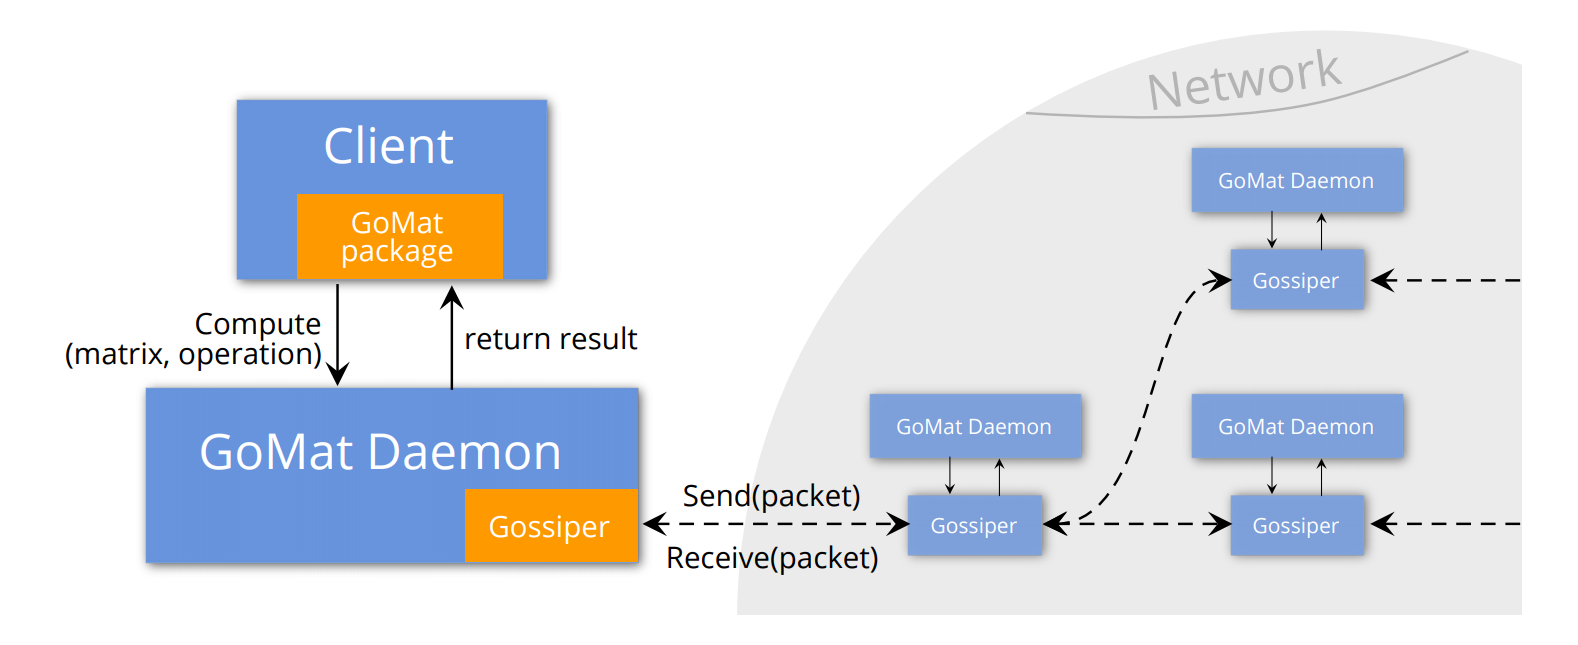
\includegraphics[width=.95\textwidth]{global_view.png}
        \caption{Global view}
        \label{glbView}
    \end{figure}
    \begin{figure}[!ht]
        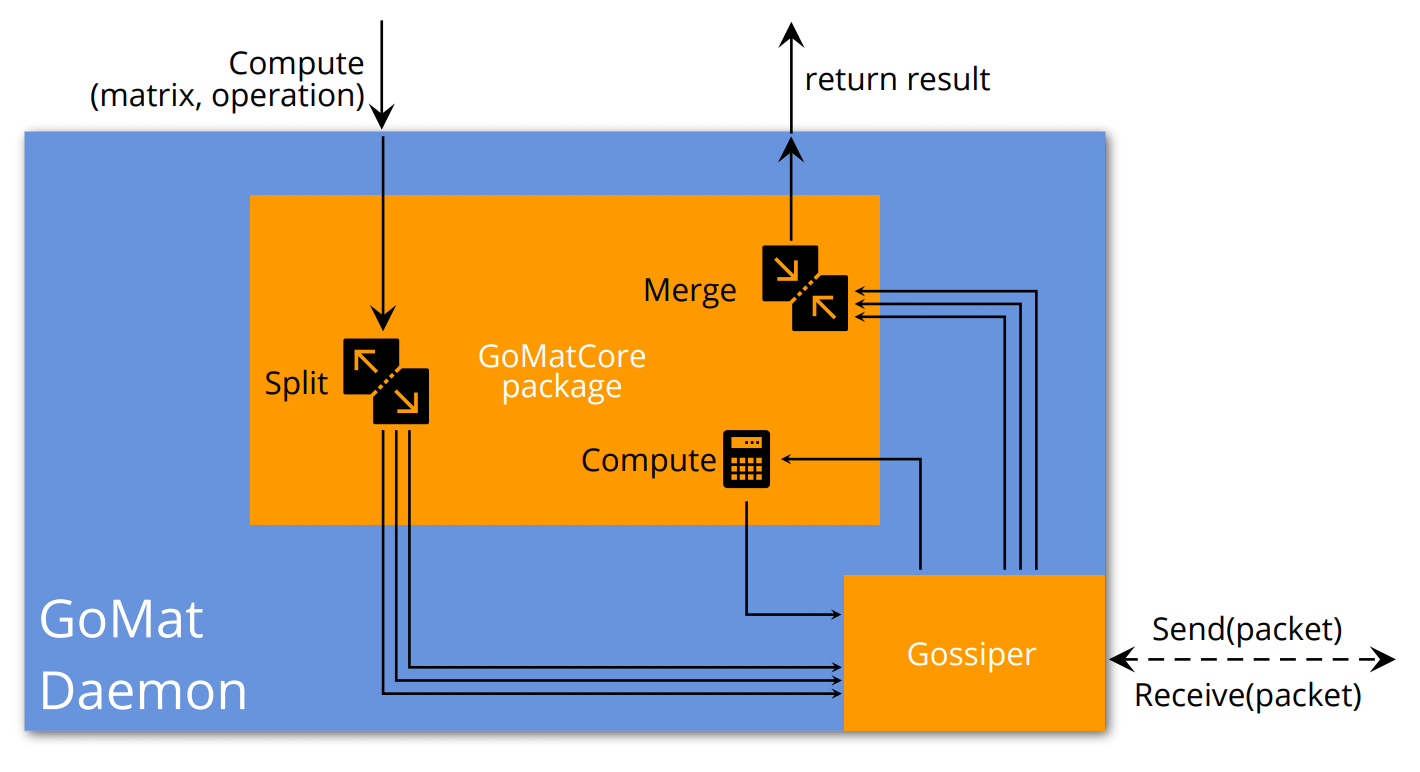
\includegraphics[width=.95\textwidth]{daemon_view.PNG}
        \caption{Daemon architecture}
        \label{daemonView}
    \end{figure}
        \subsection{Daemon}
        The creation of GoMatCore package and the demonstration application will be supervised by Kévin Carenou.

        A \Gomat peer is not a \Gossiper peer, but contains a \Gossiper peer that it uses to send and receive messages. Our \Gomat application uses the \Gossiper as a transport layer (layer 4).

        \subsubsection{GUI}
        Once the daemon is running, it is not automatically connected to a \Gomat network. The user has to open a web browser and go on \url{http://localhost:8088} (can be modified in a configuration file) to add some peers to be connected on a
    \Gomat network.

    \subsubsection{Split, merge and computation}
    When receiving a computation request from the API, the daemon splits the input matrices into smaller submatrices, to be sent to the network for computations. This submatrices are identified by their position (row/column) as a block of the original/result matrix.

    When a peer's deamon accept to compute a chunk of data, this deamon will do the computation using the \texttt{GoMatCore} package. This package implements functions computing the different operations.

    After receiving the results of the computations, the daemon merges the subresults into a result matrix. Some operations such as multiplication needs several steps to compute. In the case of multiplication, we first need to compute the multiplication between submatrices and we get the results. Then we launch the addition of block to get the result matrix.

    \subsection{API}
    The API in charge of the communication between the application and the Daemon will be implemented by Gauthier Jolly.

    Our API is a \Go package which is used to communicate with the daemon. When an application wants to compute an operation between to big matrices, he calls:\\
    \texttt{Gomat.compute(matrix1, matrix2 Matrix, operation Gomat.Operation) (result Matrix, err error)}


    This function is blocking.

    If there is no \Gomat daemon running on the computer, \texttt{Gomat.compute} returns an error.

        \subsubsection{Communications between API and Daemon}
    The application using the API and the Daemon are running on the same computer. Thus, there is no need to use the network (i.e. the loopback interface).
    We use \texttt{Inter-Process Communication (IPC) sockets} to send information between the daemon and the API.

        \subsection{Computations redistribution and failure management}
        Computations redistribution and failure management will be supervised by Matei Oltean.

        \subsubsection{Computations redistribution}
    Each gossiper doing computations has a maximum computational power, and a current one (reduced for every current computation).
    
    When a gossiper receives a computation order from the API, the following happen:
    \begin{itemize}
    \item That gossiper splits the matrices, which should be of a maximum size \texttt{self.MaximumComputationalPower}. There is a trade-off, since if the matrices are too small, there is no real gain (too much time is lost splitting and sending), and if they are too big, nobody will be able to take care of the computation. So, we decided that only the initial gossiper can split the matrices, and that they should be moderately big.
    \item Then it sends pairs of submatrices, with the operation to perform on them (as subtasks) to random alive peers or itself. They can either accept the task, or not. For each task, after a timeout, the task sent is not being taken care of, it is sent again to another random peer.
    \item When a peer receives a subtasks, it checks if it can compute it. If it is too big, it send it again to another random peer. To ensure that these messages do not keep being sent indefinitely, they have a \texttt{HopLimit} field, which is decreased every time it is sent again, and the message is discarded when it reaches 0.
    If the peer can take care of the computation, it does not start it yet, but sends a message to inform the initial node that it is ready to do so, and waits for an acknowledgement to start.
    \item For each subtask, the master node selects the first node that can take care of it as the owner of the computation and sends it a message back to inform it.
    \item Then, it waits for all the subresults, and when every computation is done, the submatrices are merged and sent to the API.
    \end{itemize}

        \subsubsection{Detecting failures}
    To manage failures, we first need to detect them. No failure detector can be perfect, but it must be eventually perfect. We also need to make sure that we do not saturate the server with ping messages to detect failures, since that could lead to other failures. Also, we do not want to suspect other nodes too early, since it is costlier to have less peers than having detected failing ones too late.
    
    We used a heuristic similar to the \textit{route flap damping} of BGP. Whenever we add a peer, we set a counter for it, starting at 0. Every \textit{timer} seconds, we send it a message and we increment the counter. Whenever we receive a status message from him, we decrement it. A peer that has a counter above a certain (small) threshold is considered to have been failed.
    
    \subsubsection{Failure management}
    When a gossiper $g$ finds that another one, $a$, has failed, it will be removed from the list of peers, the routine created to communicate with $a$ will be killed and one of the three will occur:

\begin{itemize}
\item If $a$ was doing some computation for $g$, $g$ will split the computation between its remaining peers.
\item If $g$ was doing some computation for $a$, $a$ will stop its computation, and not send the result back anymore.
\item In any other case, nothing more will be done.
\end{itemize}

    \subsubsection{Making the system more resilient}
    If a gossiper $g$ receives a task and has enough idle peers, it can redistribute some of it amongst them. There must be some wait time (maybe they have all received subtasks from the same job, but because of delays, $g$ still sees them as idle).
In that case, the ‘master’ peer must be informed of their computations, they will be added to its peers, and as for others, it must now detect their failures.

    Then, if $g$ crashes, not all of the computations sent to him will have to be redone, since some subtasks are now processed by its peers.

    The master node will also be able to add gossipers to its list of known peers, and the network will be more robust.
    
    Also, since the failure detector is not perfect, there are timeouts on every routine involving other peers. Upon a short timeout, the task will be dispatched to another peer.

    \section{Evaluation Plan}
    First, we need to be sure, that the matrix splitting, merging, and the operations on them behave as they should.

    To test the implementation of these operations, unit tests using the \texttt{testing} package available in golang will be written and launched after every change of any of the operations. Also, after being sure that they work locally, we will also test them within a small network.

    Since most of the tests will be run through the API, we must also check that when \texttt{Gomat.compute} is executed, the correct tasks are run in the background.

~~

    Since the message spreading is built on top of Peerster, it should work and is already tested. Obviously, the messages sent for computations and failure detection are different from GossipPackets, but we will check if everything works when testing our parts of the program.

~~

    For the failure detection, we will have to check two things (and also adapt the timeout parameters accordingly): that if a peer fails, the other detect it fast, and that there a very few false positives (i.e. that a node is seen as having failed, while it still runs fine). We will simulate small networks, with failing nodes (i.e. deconnexions), and check the reactions of the remaining gossipers.

    We will also check that when a node receives a message, it always adds the sender to its list of known peers, by sending blank messages (we must also be sure that a message not well formatted is discarded, instead of making the node thread crash).

~~

    While all those tests will be running, we will have a GUI running, and we will check that all the informations displayed are correct.

    \section{Conclusion}
    These specifications are meant to change, since it is only a second draft.

    For example, a function of preference should be added. The sizes of the matrices sent for computations should depend on the computation power of the gossiper, its response time,~etc. But for that, we would also need to optimise the splitting and merging parts, in order to be able to efficiently merge submatrices of different sizes.
\end{document}
